\section{src/system.cpp File Reference}
\label{system_8cpp}\index{src/system.cpp@{src/system.cpp}}
{\tt \#include \char`\"{}system.hpp\char`\"{}}\par


Include dependency graph for system.cpp:\begin{figure}[H]
\begin{center}
\leavevmode
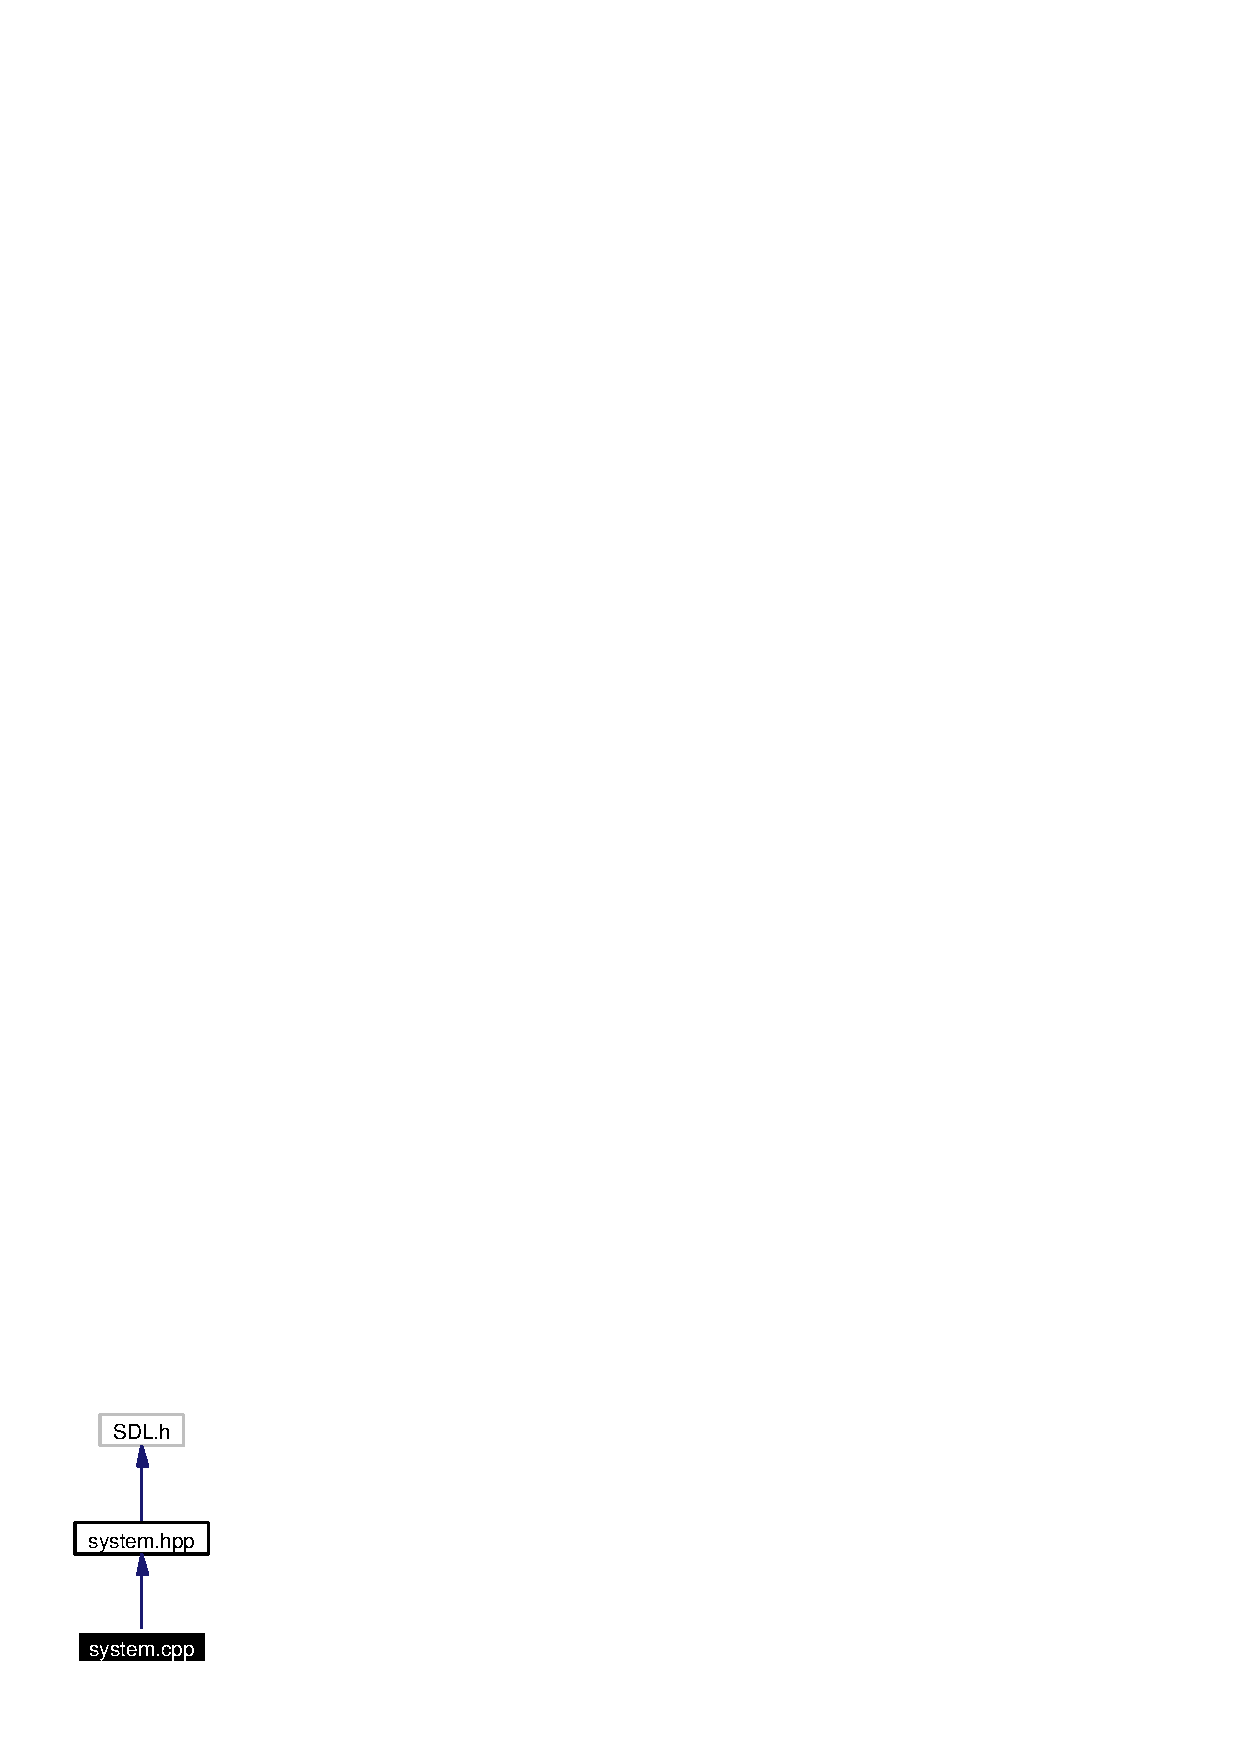
\includegraphics[width=50pt]{system_8cpp__incl}
\end{center}
\end{figure}
\subsection*{Variables}
\begin{CompactItemize}
\item 
bool {\bf main\-Loop\-Enabled}
\item 
bool {\bf sim\-Loop\-Enabled}
\item 
bool {\bf gui\-Loop\-Enabled}
\end{CompactItemize}


\subsection{Variable Documentation}
\index{system.cpp@{system.cpp}!guiLoopEnabled@{guiLoopEnabled}}
\index{guiLoopEnabled@{guiLoopEnabled}!system.cpp@{system.cpp}}
\subsubsection{\setlength{\rightskip}{0pt plus 5cm}bool {\bf gui\-Loop\-Enabled}}\label{system_8cpp_a2}


\index{system.cpp@{system.cpp}!mainLoopEnabled@{mainLoopEnabled}}
\index{mainLoopEnabled@{mainLoopEnabled}!system.cpp@{system.cpp}}
\subsubsection{\setlength{\rightskip}{0pt plus 5cm}bool {\bf main\-Loop\-Enabled}}\label{system_8cpp_a0}


\index{system.cpp@{system.cpp}!simLoopEnabled@{simLoopEnabled}}
\index{simLoopEnabled@{simLoopEnabled}!system.cpp@{system.cpp}}
\subsubsection{\setlength{\rightskip}{0pt plus 5cm}bool {\bf sim\-Loop\-Enabled}}\label{system_8cpp_a1}


